\documentclass{comjnl}

\usepackage[utf8]{inputenc}       
\usepackage[slovene]{babel}
\usepackage{booktabs}
\usepackage[table,xcdraw]{xcolor}
\usepackage{caption}


\captionsetup{
  singlelinecheck = false, format= hang, justification=raggedright
}

%% These two lines are needed to get the correct paper size
%% in TeX Live 2016
\let\pdfpageheight\paperheight
\let\pdfpagewidth\paperwidth

%\copyrightyear{2018} \vol{00} \issue{0} \DOI{000}

\begin{document}
\author{João Bettencourt}
\title{Brute-force, Dictionary Attacks and Mitigation}
\affiliation{Fakulteta za elektrotehniko, računalništvo in informatiko, Univerza v Mariboru} \email{joao.bettencourt@um.si}

\shortauthors{J. Bettencourt}
 

\keywords{Password; BruteForce; Dictionary Attacks; Mitigation}


\begin{abstract}
The increasing reliance on digital systems in contemporary society has elevated the importance of robust security measures. One of the most persistent threats to digital security is the brute-force and dictionary attack, which exploits weak passwords to compromise systems. This paper explores these attack techniques, their mechanisms, and their impact on cybersecurity. By understanding the principles behind brute-force and dictionary attacks, we can identify vulnerabilities in password systems and propose effective mitigation strategies. The choice of this topic stems from its relevance in today's world, where the implementation of security standards and practices has become crucial for safeguarding sensitive information. The study also emphasizes the need for stronger authentication methods and awareness to protect against evolving attack techniques. Through theoretical exploration and practical demonstration using tools like Kali Linux, this work aims to highlight not only the risks posed by these attacks but also actionable measures to enhance digital security.
\end{abstract}

\maketitle


\section{Introduction}
\label{Sec:Sklicnapoglavje}
The purpose of the introduction of an article or other research text is to introduce the reader to the research field, to present the purpose and meaning of the paper. As a rule, it consists of two parts: in the first part, you first give a reason for choosing a topic, in which it is not appropriate to write that you decided on the topic because you like it or it attracted you; instead, try to stay as objective as possible and write down why the chosen topic is important. Briefly present the topic and highlight its main or key features. In the second part, briefly describe the structure of the article. You can do this by summarizing each chapter of the article, such as: "The next chapter lists the language and format requirements for writing an article. The third chapter provides important guidance on citing sources" \cite{VomBrocke2015}.

\section{Language, size, and format} 

The article must be written in the English language and must be linguistically sound. Its length should be between 5 and 10 pages. Shorter or longer papers will be penalized based on the number of pages under/over the limit. 

The lines should be spaced exactly one space apart. There should be a 6 pt space before each paragraph. Do not leave extra blank lines between paragraphs. The spacing between paragraphs should be 18 pt before and 6 pt after chapters, and 12 pt before and 6 pt after subchapters. Start writing paragraphs on the left and do not make indentations to the right. The text should be aligned in a block (center alignment, i.e. left and right margin aligned). Letter size should be 12, Times New Roman font. The entire text should be aligned in two columns. You can follow the given template to achieve this.

\subsection{Figures, lists, and tables}

Within the text, you must refer at least once to the displayed figures, tables and/or equations. Example: The figure \ref{fig:model} shows a theoretical research model. The \ref{fig:registration} image shows the registration button.

\begin{figure}
\centering
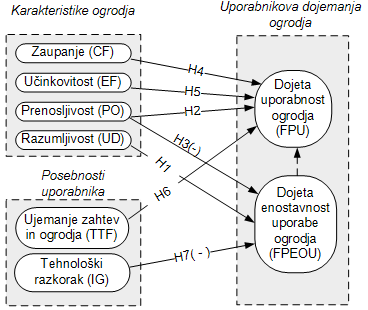
\includegraphics[width=0.5\textwidth]{teoreticni_model}
\caption{Title of the figure}\label{fig:model}
\end{figure}

Use the \textit{itemize} command to create a list as follows:

\begin{itemize}
     \item The first enumeration element,
     \item Second enumeration element and
     \item The third enumeration element.
\end{itemize}

Numbering is also used in the same way as enumeration, using the \textit{enumerate} command. You can see an example below:

\begin{enumerate}
     \item The first numbering element,
     \item Second numbering element and
     \item The third numbering element.
\end{enumerate}

Tables must have a description that unambiguously describes the data presented in the table. It is also necessary to refer to all the tables in the article.

This document is written in the format that the article should be in, and is useful as a template for writing with \LaTeX in the Overleaf environment.

\begin{table}[t]
\caption{Title of the small table}
\label{tab:malatabela}
\begin{tabular}{|l|l|l|}
\hline
\rowcolor[HTML]{656565} 
{\color[HTML]{FFFFFF} Variable} & {\color[HTML]{FFFFFF} Coefficient} & {\color[HTML]{FFFFFF} P} \\ \hline
Gender & 4.31 & 0.001 \\ \hline
Age & 2.33 & 0.005 \\ \hline
GCS1 & 8.24 & 0.001 \\ \hline
GCS2 & 9.12 & 0.001 \\ \hline
\end{tabular}
\end{table}

Praesent pellentesque, elit id varius sagittis, urna leo viverra magna, ac consectetur sapien justo eu sapien. As has been shown (Laramee 2009) Cras viverra nulla in arcu posuere id sollicitudin leo sollicitudin. Suspendisse gravida odio vel arcu ltrices ultrices. Integer elementum elit rhoncus lectus gravida imperdiet. Nulla et lorem lacus, in commodo arcu. Vivamus a nisl elit. Curabitur nisl nisi, laoreet in tristique ac, facilisis eu justo. Proin consequat metus id libero consectetur ultricies. Phasellus commodo adipiscing posuere \cite{Figl2013}.

Nam augue erat, posuere eu condimentum ut, lacinia eget eros. Nam sit amet nibh magna, hendrerit ultrices urna. Morbi id augue dui. Donec eros ligula, mattis eu rhoncus id, molestie ut nulla. 
Eenean vulputate, mi eu ultrices ullamcorper, neque ligula varius diam, a luctus ante quam vitae felis. Praesent dignissim aliquet augue nec interdum. Pellentesque nec fermentum neque. Donec libero sem, sagittis ac pretium quis \cite{Genon2011}.

\label{Sec:Sklicnapodpoglavje}

Praesent pellentesque, elit id varius sagittis, urna leo viverra magna, ac consectetur sapien justo eu sapien. As has been shown (Laramee 2009) Cras viverra nulla in arcu posuere id sollicitudin leo sollicitudin. Suspendisse gravida odio vel arcu ltrices ultrices. Integer elementum elit rhoncus lectus gravida imperdiet. Nulla et lorem lacus, in commodo arcu. Vivamus a nisl elit. Curabitur nisl nisi, laoreet in tristique ac, facilisis eu justo. Proin consequat metus id libero consectetur ultricies. Phasellus commodo adipiscing posuere.

\section{Important instructions} 

In the list of resources at the end of the article, list all the resources that you used to create the article (scientific and professional articles, conference proceedings, books, websites, etc.) that you refer to as part of the assignment. Detailed instructions for citing sources are provided in the next subsection.

\begin{figure}[b]
\centering

\includegraphics[width=2in]{registracija}
\caption{Title of the figure \cite{Mick1986}}\label{fig:registracija}
\end{figure}

\subsection{Citing}

You should use references to refer to the resources in the article. By referring, you indicate that a particular thought, a particular procedure, or a particular claim is not yours, but you have read it somewhere and are quoting it. If you are literally copying the source, you need to put it in quotation marks and state the source at the end. However, if you are summarizing the source, it is not necessary to use quotation marks, but you must refer to the source at the end of the sentence.

It makes sense to edit the resources in an external file (.bib), using the Bibtex reference format. Referencing the sources is mandatory! To reference a source, use the \textit{cite} command to specify a key that uniquely identifies the source in the source list. The sources are also collected and listed in a list at the end of the document. Each listed item should include all relevant information about the mentioned source. The References section provides examples of references to a book, article, and online resource; for other types of resources you can refer to the \LaTeX documentation.

Nam augue erat, posuere eu condimentum ut, lacinia eget eros. Nam sit amet nibh magna, hendrerit ultrices urna. Morbi id augue dui. Donec eros ligula, mattis eu rhoncus id, molestie ut nulla. Aenean vulputate, mi eu ultrices ullamcorper, neque ligula varius diam, a luctus ante quam vitae felis. Praesent dignissim aliquet augue nec interdum. Pellentesque nec fermentum neque. Donec libero sem, sagittis ac pretium quis, ultrices nec massa. Donec sed felis felis. Vestibulum sed turpis felis.
Figure \ref{fig:registracija} showcases a registration button. 


\section{Chapter} 

\begin{table*} %široke tabele so zmeraj prikazane na dnu ali na vrhu strani
\captionsetup{justification=raggedright}
\caption{Title of a large table}
\label{tab:sirokatabela}
\begin{tabular}{>{\raggedright\arraybackslash}m{2.7cm}>{\raggedright\arraybackslash}m{3.3cm}>{\raggedright\arraybackslash}m{3.3cm}>{\raggedright\arraybackslash}m{3cm}>{\raggedright\arraybackslash}m{3.3cm}}
\rowcolor[HTML]{656565} 
{\color[HTML]{FFFFFF} \textbf{Authors}} & {\color[HTML]{FFFFFF} \textbf{Constructs}} & {\color[HTML]{FFFFFF} \textbf{Context IT}} & {\color[HTML]{FFFFFF} \textbf{Method}} & {\color[HTML]{FFFFFF} \textbf{Conclusions}} \\ 
Davis & PU, PEOU, U & PROFs, XEDIT, Chart-Master, Pendraw & Survey, experiment &   PEOUàU \\ \hline
Davis, Bagozzi in Warshaw & PU, PEOU, A, BI, U & WriteOne & Experiment & PEOUàPU, PUàA, PEOUàA, AàBI, PUàBI, BIàU \\ \hline
Haynes in Thies & PU, PEOU, U & Automatic pager & Survey & PUàU, PEOUàU \\ \hline
Mathieson & EV, PU, PEOU, A, BI, U & Table, calculator & Experiment & PUàU,   PEOUàU \\ \hline
\end{tabular}
\end{table*}



Nam augue erat, posuere eu condimentum ut, lacinia eget eros. Nam sit amet nibh magna, hendrerit ultrices urna. Morbi id augue dui. Donec eros ligula, mattis eu rhoncus id, molestie ut nulla. Aenean vulputate, mi eu ultrices ullamcorper, neque ligula varius diam, a luctus ante quam vitae felis. Praesent dignissim aliquet augue nec interdum. Pellentesque nec fermentum neque. Donec libero sem, sagittis ac pretium quis, ultrices nec massa. Donec sed felis felis. Vestibulum sed turpis felis \cite{ZZPPZ}.

Explanation: Coefficients are beta coefficients of logistic regression. GCS1 and GCS2 are determined on clinical examination before surgery. Nam augue erat, posuere eu condimentum ut, lacinia eget eros. Nam sit amet nibh magna, hendrerit ultrices urna. Morbi id augue dui. Donec eros ligula, mattis eu rhoncus id, molestie ut nulla. Aenean vulputate, mi eu ultrices ullamcorper, neque ligula varius diam, a luctus ante quam vitae felis. Praesent dignissim aliquet augue nec interdum. Pellentesque nec fermentum neque. Donec libero sem, sagittis ac pretium quis, ultrices nec massa. Donec sed felis felis. Vestibulum sed turpis felis \cite{iib}.
Explanation: Coefficients are beta coefficients of logistic regression. GCS1 and GCS2 are determined on clinical examination before surgery \footnote{Footnote}.




\section{Conclusion} 
\label{Conclusions}
The article ends with a conclusion in which you once again state the issues you have described, the main features and your observations or results. In the end, you describe what you presented in the whole document and what you "achieved" with the presentation, so you describe the results of your work and the new insights you have gained through research in the field. You can also indicate opportunities for further research and work.

Nam augue erat, posuere eu condimentum ut, lacinia eget eros. Nam sit amet nibh magna, hendrerit ultrices urna. Morbi id augue dui. Donec eros ligula, mattis eu rhoncus id, molestie ut nulla. Aenean vulputate, mi eu ultrices ullamcorper, neque ligula varius diam, a luctus ante quam vitae felis. Praesent dignissim aliquet augue nec interdum. Pellentesque nec fermentum neque. Donec libero sem, sagittis ac pretium quis, ultrices nec massa. Donec sed felis felis. Vestibulum sed turpis felis.


\begin{itemize}
    \item Pellentesque nec fermentum neque.
    \item Nam sit amet nibh magna, hendrerit
    \item Aenean vulputate, mi eu ultrices
\end{itemize}
Eenean vulputate, mi eu ultrices ullamcorper, neque ligula varius diam, a luctus ante quam vitae felis. Praesent dignissim aliquet augue nec interdum. Pellentesque nec fermentum neque. Donec libero sem, sagittis ac pretium quis, ultrices nec massa. Donec sed felis felis. Vestibulum sed turpis felis 





\bibliographystyle{compj}
\bibliography{literatura}


\end{document}